% Created 2020-07-16 Thu 20:03
% Intended LaTeX compiler: pdflatex
\documentclass[letter]{article}
\usepackage[utf8]{inputenc}
\usepackage[T1]{fontenc}
\usepackage{graphicx}
\usepackage{grffile}
\usepackage{longtable}
\usepackage{wrapfig}
\usepackage{rotating}
\usepackage[normalem]{ulem}
\usepackage{amsmath}
\usepackage{textcomp}
\usepackage{amssymb}
\usepackage{capt-of}
\usepackage{hyperref}
\usepackage{multicol}
\usepackage[margin=1.3in]{geometry}
\setlength{\columnsep}{1cm}
\usepackage{palatino}
\fontfamily{ppl}\selectfont
\usepackage[spanish]{babel}
\renewcommand{\baselinestretch}{1.5}
\usepackage{fancyhdr}
\fancyhf{}
\pagestyle{fancy}
\lhead{\hleft}
\rhead{\hright}
\cfoot{\thepage}
\renewcommand{\headrulewidth}{1pt}
\renewcommand{\footrulewidth}{0pt}
\newcommand{\hleft}{Programación Multimedial}
\newcommand{\hright}{INF 324}
\setlength{\parindent}{0cm}
\author{Jesus Rodolfo Izurieta Veliz}
\date{\today}
\title{INF 324 - Informe de desarrollo primer parcial}
\hypersetup{
 pdfauthor={Jesus Rodolfo Izurieta Veliz},
 pdftitle={INF 324 - Informe de desarrollo primer parcial},
 pdfkeywords={},
 pdfsubject={},
 pdfcreator={Emacs 26.3 (Org mode 9.4)}, 
 pdflang={Spanish}}
\begin{document}

\maketitle
Para este proyecto usaremos la biblioteca codeigniter para desarrollar en php,
para la base de datos usaremos mariadb, un motor de base de datos open source
basado en mysql. El proyecto estará organizado en contenedores docker, para
facilitar su distribución y replicar su funcionamiento sin tener que lidiar con
problemas de versiones ni configuraciones extra para el funcionamiento del
proyecto.

\section{Configuración del proyecto}
\label{sec:org0569705}
La estructura del proyecto estará definida por el archivo \texttt{docker-compose.yml},
en el que indicaremos las imágenes de docker que se usarán para el proyecto, en
este caso, usaremos contenedores de codeigniter y mariadb.

\begin{verbatim}
version: '2'
services:
  myapp:
    image: 'docker.io/bitnami/codeigniter:3-debian-10'
    ports:
      - '8000:8000'
    volumes:
      - '.:/app'
    depends_on:
      - mariadb
  mariadb:
    image: 'docker.io/bitnami/mariadb:10.3-debian-10'
    ports:
      - '3306:3306'
    volumes:
      - './mysql:/bitnami/mariadb'
    environment:
      - ALLOW_EMPTY_PASSWORD=yes
\end{verbatim}

\section{Base de datos}
\label{sec:orgb14ae8d}
Después de inicializar el proyecto con docker, necesitaremos crear la base de
datos, nos conectamos al contenedor de mariadb con el comando:

\texttt{docker exec -it 65bdcb8d72f1 bash}

Donde \texttt{65bdcb8d72f1} es el código del contenedor, que puede obtenerse con el
comando \texttt{docker ps} cuando el proyecto está ejecutándose.

\subsection{Creación de tablas}
\label{sec:orgd3f31bc}
En la línea de comandos, iniciamos una sesión en mysql con el comando:

\texttt{mysql -u root -p}

Se nos pedirá una contraseña, que será la que tenemos configurada en el archivo
\texttt{docker-compose.yml} o en su defecto, nos permitirá ingresar sin una contraseña
la primera vez.

Creamos un usuario con el comando

\texttt{GRANT ALL PRIVILEGES ON *.* TO 'username'@'localhost' IDENTIFIED BY 'password';}

Poniendo el nombre del usuario en lugar de \guillemotleft{}username\guillemotright{} y la contraseña en lugar
de \guillemotleft{}password\guillemotright{}. En este caso creamos el usuario admin.

Ahora saldremos de mysql con \texttt{\textbackslash{}q}, y volveremos a ingresar con el usuario y
contraseña recientemente creados.

\texttt{mysql -u admin -p}

Ahora crearemos la base de datos y la seleccionaremos para crear las tablas en
ella.

\texttt{CREATE DATABASE academico;}
\texttt{USE academico;}

ahora crearemos las siguientes tablas:

\textbf{Tabla USUARIO}

\begin{center}
\begin{tabular}{lllll}
Campo & Tipo de dato & Longitud & PK & Descripción\\
\hline
pk & int &  & si & Llave primaria\\
dni & int &  &  & CI del usuario\\
password & varchar & 40 &  & Clave para ingresar\\
photo & varchar & 200 &  & Url de la fotografía\\
\end{tabular}
\end{center}

Con la consulta:

\begin{verbatim}
CREATE TABLE usuario
(
    pk int unsigned not null auto_increment,
    dni varchar(20) not null,
    password varchar(40) not null,
    photo varchar(200),
    primary key (pk)
);
\end{verbatim}

\textbf{Tabla IDENTIFICADOR:}

\begin{center}
\begin{tabular}{llrll}
Campo & Tipo de dato & Longitud & PK & Descripción\\
\hline
pk & int &  & si & Llave primaria\\
user\textsubscript{pk} & int &  &  & Llave foránea de usuario\\
dni & int & 20 &  & CI del usuario\\
first\textsubscript{name} & varchar & 100 &  & Nombres\\
last\textsubscript{name} & varchar & 100 &  & Apellidos\\
birth\textsubscript{date} & date &  &  & Fecha de nacimiento\\
residence & varchar & 10 &  & Código del lugar de residencia\\
\end{tabular}
\end{center}

Con la consulta:

\begin{verbatim}
CREATE TABLE identificador
(
    pk int unsigned not null auto_increment primary key,
    user_pk int unsigned,
    dni varchar(20) not null,
    first_name varchar(100),
    last_name varchar(100) not null,
    birth_date date,
    residence varchar(10),
    foreign key (user_pk) REFERENCES usuario(pk)
);
\end{verbatim}

\textbf{Tabla NOTAS}

\begin{center}
\begin{tabular}{lllll}
Campo & Tipo de dato & Longitud & PK & Descripción\\
\hline
pk & int &  & si & Llave primaria\\
user\textsubscript{pk} & int &  &  & Llave foránea de usuario\\
matter & varchar & 50 &  & Materia\\
score & int &  &  & Calificación\\
\end{tabular}
\end{center}

Con la consulta:

\begin{verbatim}
CREATE TABLE notas
(
    pk int unsigned not null auto_increment,
    user_pk int unsigned,
    dni varchar(20) not null,
    matter varchar(50),
    score int,
    primary key (pk),
    foreign key (user_pk) REFERENCES usuario(pk)
);
\end{verbatim}

Podremos comprobar que las tablas se crearon con el comando \texttt{show tables;}, que
nos mostrará una lista de las tablas de nuestra base de datos.

\section{Desarrollo}
\label{sec:org5a5ee58}
El proyecto consta de dos secciones para resolver los dos problemas propuestos
en el enunciado, la página de perfil de usuario, que mostrará la foto del
usuario y la parte de notas, donde se mostrará el contenido de la tabla notas.

\section{Modelos}
\label{sec:org13103e1}
Codeigniter nos permite abstraer los datos de una base de datos y las acciones
que podemos realizar sobre ellas mediante modelos que definimos por cada tabla
de la base de datos.

\subsubsection{Usuario}
\label{sec:org61c9fef}
Definimos el modelo usuario

\section{Vistas}
\label{sec:org9104397}
\subsection{Inicio de sesión}
\label{sec:org2a13731}
Para el inicio de sesión se ingresa en la dirección raíz (/) y si no se tiene
una sesión iniciada, se mostrará el formulario de inicio de sesión. En caso de
tener una sesión, el usuario podrá acceder automáticamente a su página de
perfil, donde se mostrará su foto y la opción de cambiar el color de la página.

Para esto, empezaremos por definir los modelos que representarán a las tablas de
la base de datos.

Se puede acceder a esta vista mediante la url \texttt{/login} para iniciar sesión, el
sistema nos llevará a la url \texttt{/profile} si el inicio de sesión es exitoso

\subsection{Lista de notas}
\label{sec:org46a9e3d}
La vista del listado de notas muestra la cantidad de aprobados en la base de
datos \texttt{notas}, se contará en la consulta a cualquier entrada de la base de datos
con una nota igual o mayor a 51.

Se puede acceder a esta vista mediante la url \texttt{/scores}, donde se mostrará la
cantidad de aprobados.

Podremos verificar los datos de usuarios en la base de datos:

\begin{center}
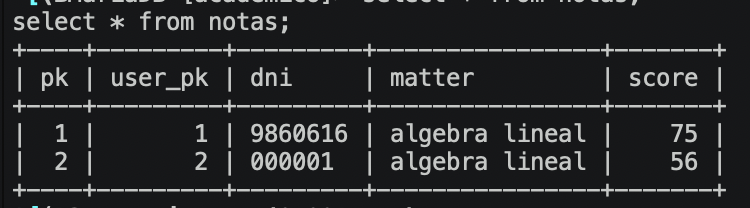
\includegraphics[width=.9\linewidth]{./img/scoredb.png}
\end{center}

\section{Pruebas}
\label{sec:org28bb55f}
\subsection{Perfil de usuario}
\label{sec:org5b3e4d1}
Ingresamos a la dirección \texttt{/login} e ingresamos con el CI \texttt{9860616} y la
contraseña \texttt{12345678x}.

\begin{center}
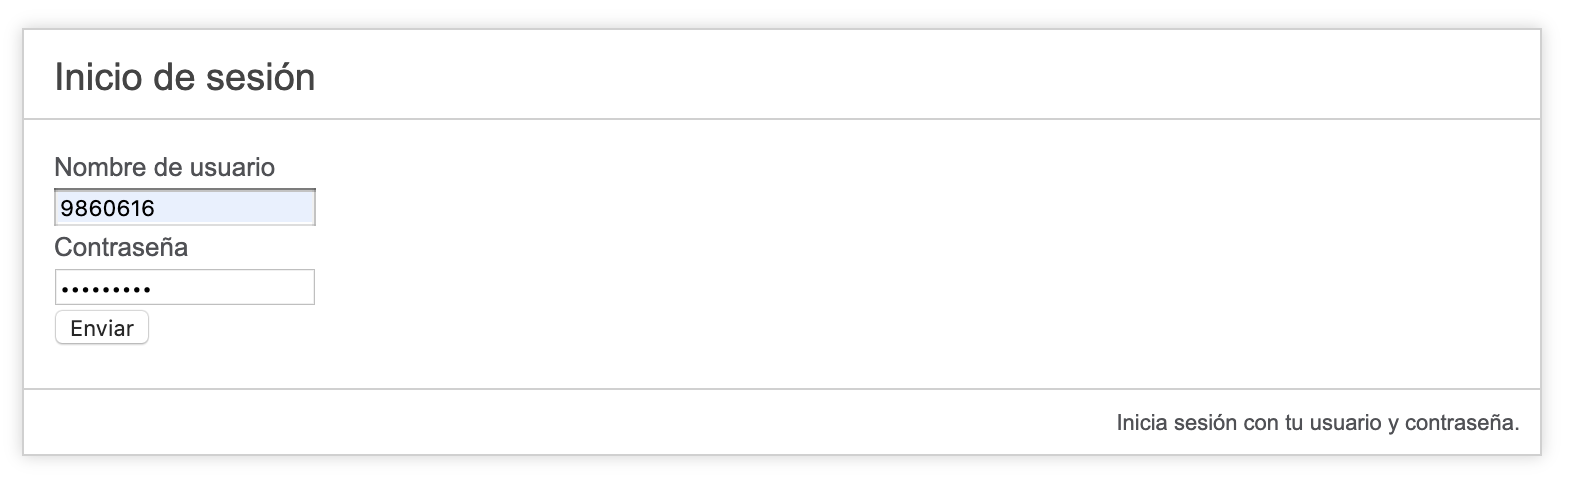
\includegraphics[width=.9\linewidth]{./img/login.png}
\end{center}

Luego de esto, iniciaremos sesión y podremos acceder a la página de perfil.

\begin{center}
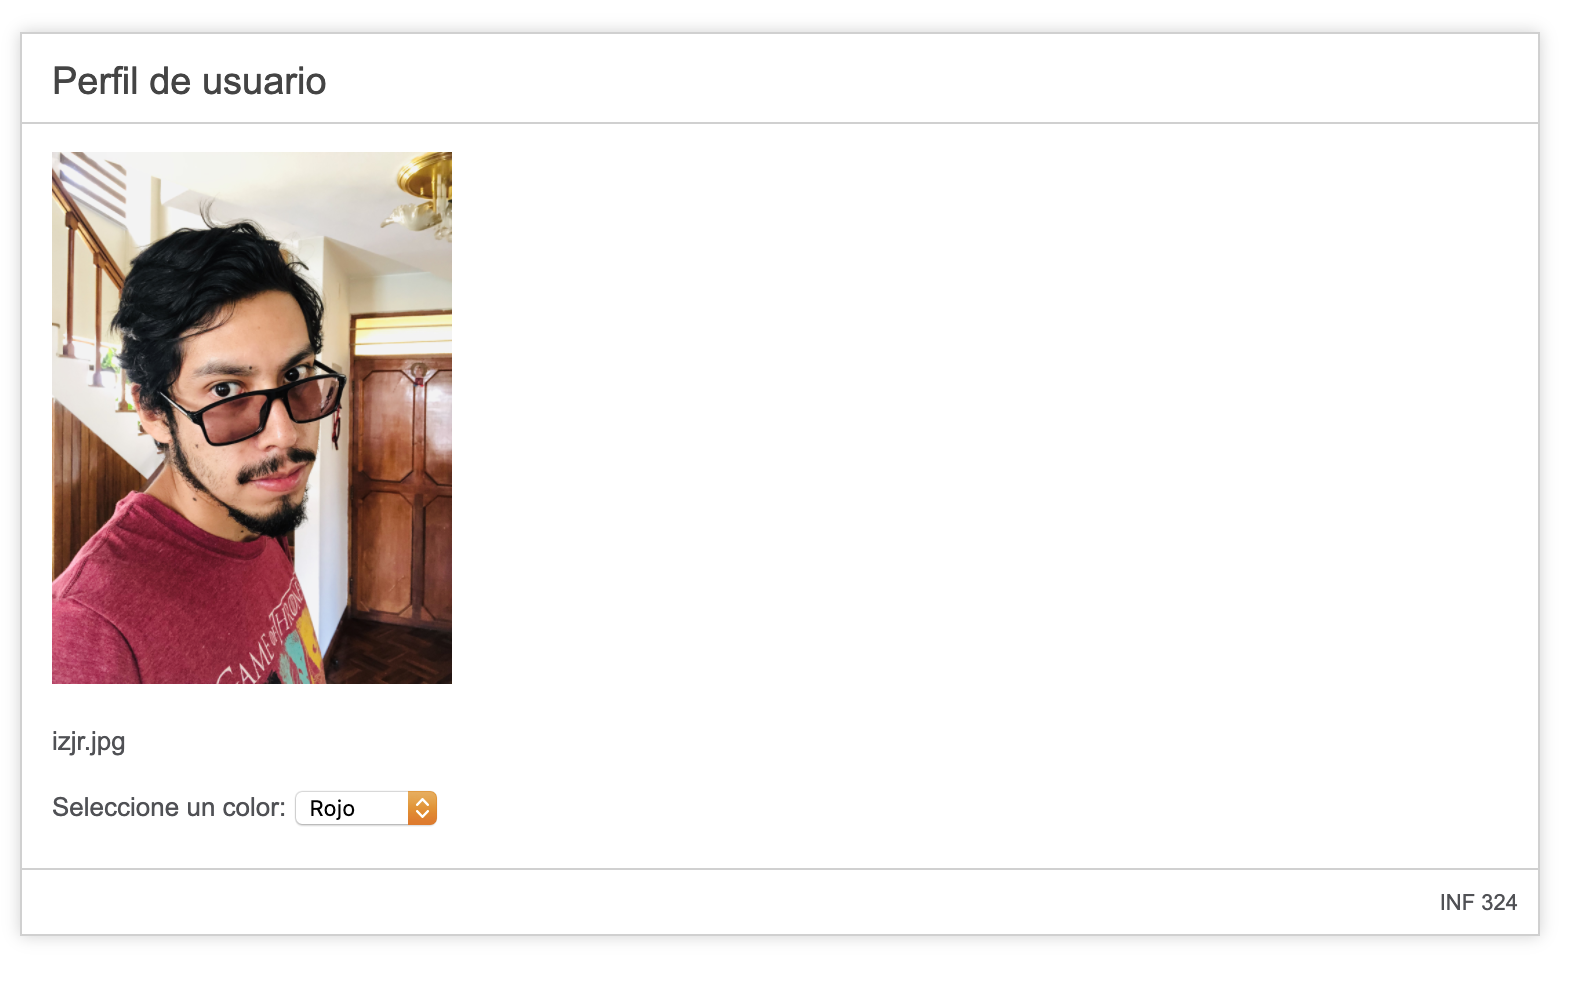
\includegraphics[width=.9\linewidth]{./img/perfil.png}
\end{center}

En la página de perfil veremos detalles del usuario y también un select que nos
permitirá cambiar el color de la página, si seleccionamos otro color, veremos el
cambio.

\begin{center}
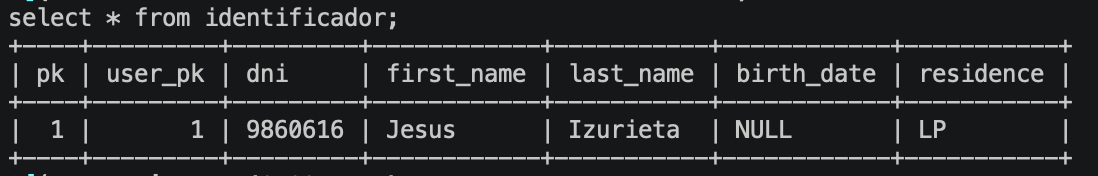
\includegraphics[width=.9\linewidth]{./img/iden.png}
\end{center}

\subsection{Notas}
\label{sec:orgf1bb77f}
Ingresamos a la dirección \texttt{/scores} podremos ver una lista de las materias aprobadas.

\begin{center}
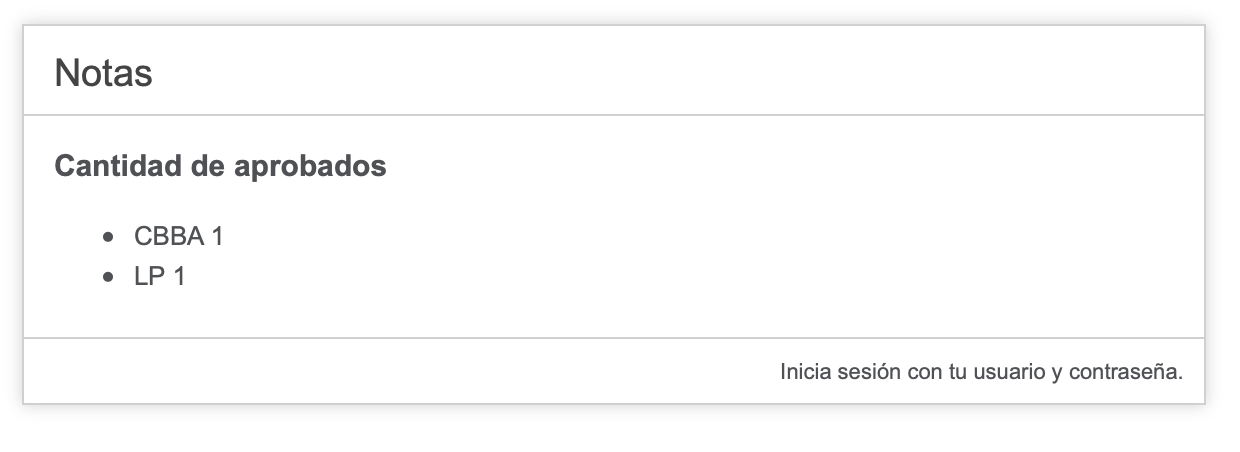
\includegraphics[width=.9\linewidth]{./img/score.png}
\end{center}

Podremos comprobar que el conteo es correcto comparando con la consulta directa
a la base de datos:

\begin{center}
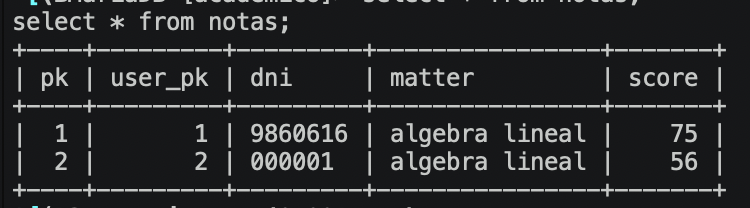
\includegraphics[width=.9\linewidth]{./img/scoredb.png}
\end{center}
\end{document}
